\section{Spark::Sp\-Grid\-Sg Class Reference}
\label{classSpark_1_1SpGridSg}\index{Spark::SpGridSg@{Spark::SpGridSg}}
{\tt \#include $<$Sp\-Grid\-Sg.h$>$}

Inheritance diagram for Spark::Sp\-Grid\-Sg:\begin{figure}[H]
\begin{center}
\leavevmode
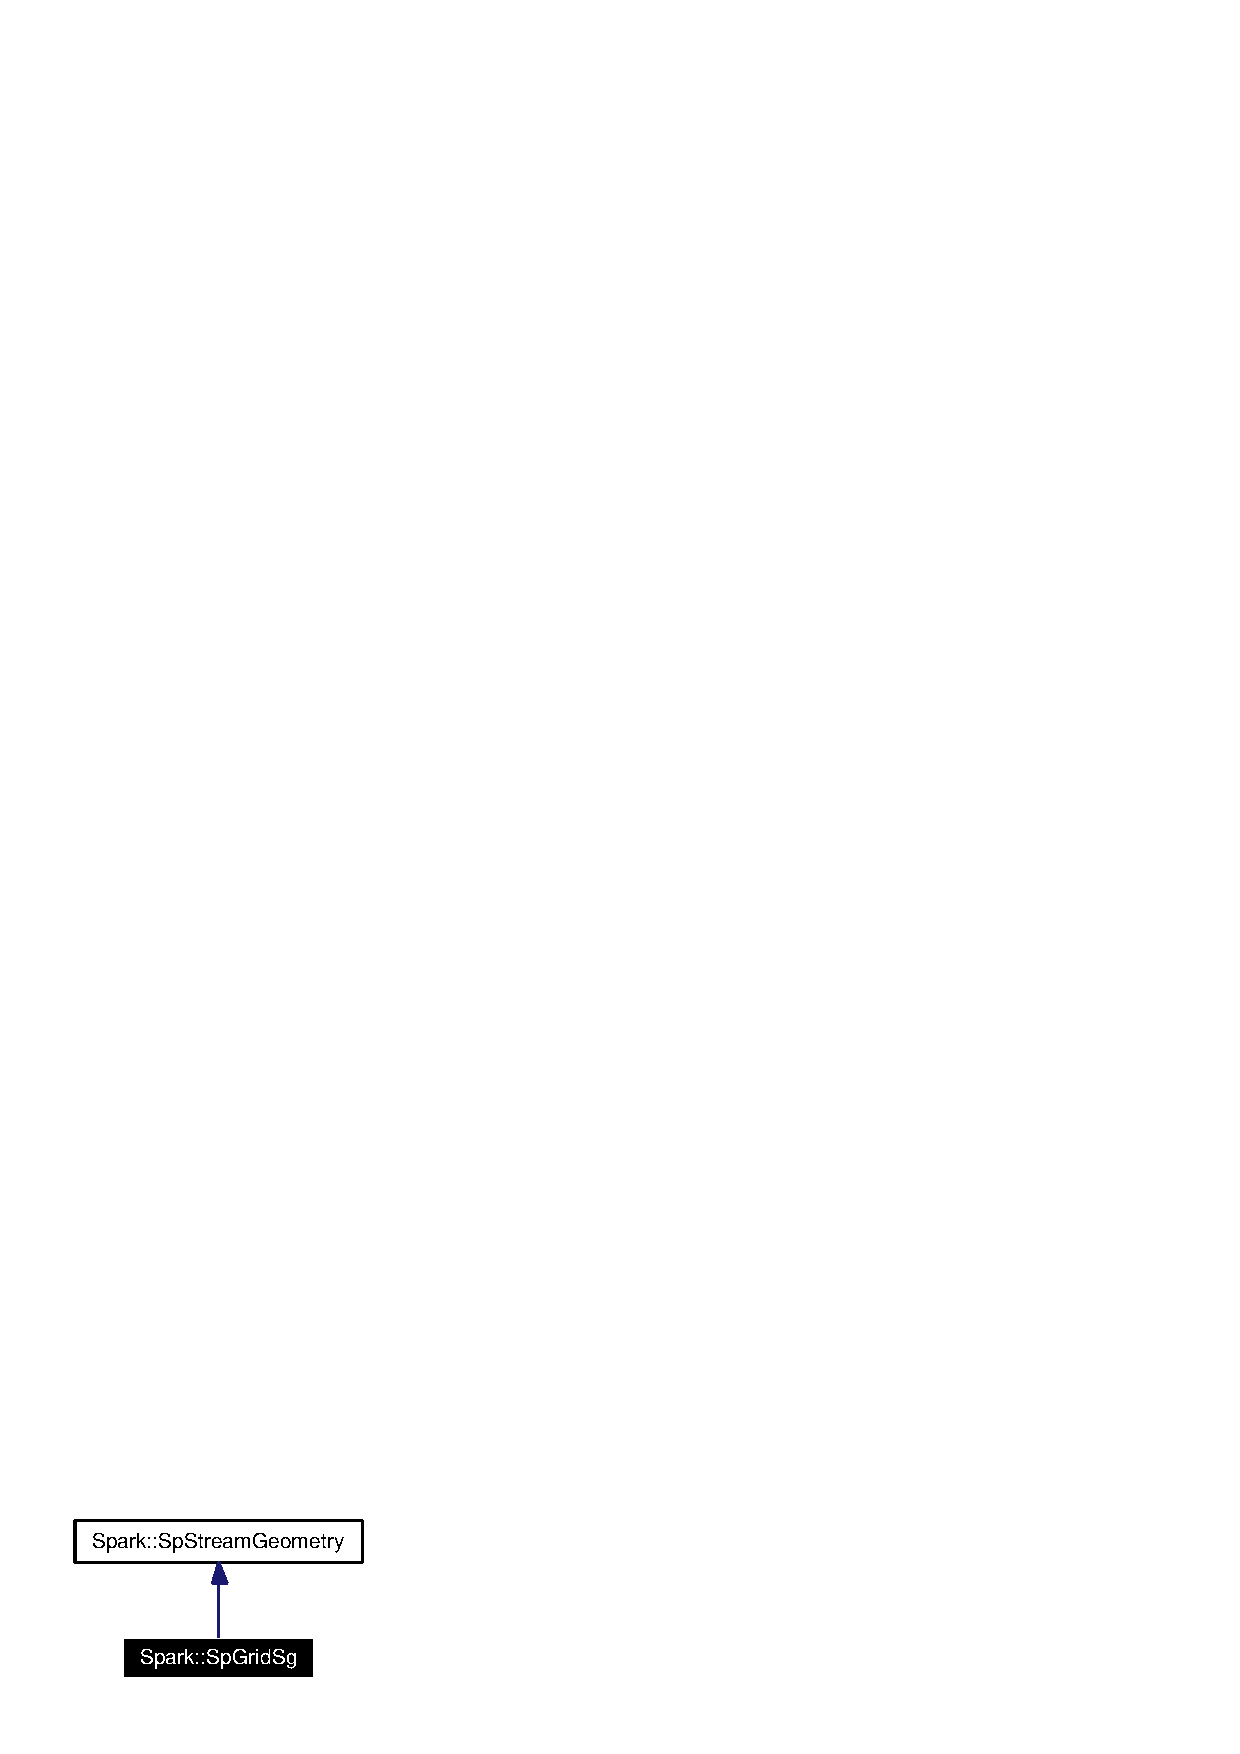
\includegraphics[width=87pt]{classSpark_1_1SpGridSg__inherit__graph}
\end{center}
\end{figure}
Collaboration diagram for Spark::Sp\-Grid\-Sg:\begin{figure}[H]
\begin{center}
\leavevmode
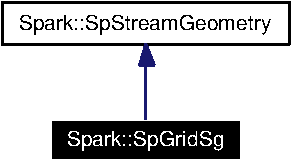
\includegraphics[width=87pt]{classSpark_1_1SpGridSg__coll__graph}
\end{center}
\end{figure}


\subsection{Detailed Description}
Multi-resolution grid-based stream geometry. 

Definition at line 33 of file Sp\-Grid\-Sg.h.\subsection*{Public Member Functions}
\begin{CompactItemize}
\item 
{\bf Sp\-Grid\-Sg} (int i\-Rows=10, int i\-Cols=10, float f\-Min\-X=-1.0f, float f\-Min\-Y=-1.0f, float f\-Max\-X=1.0f, float f\-Max\-Y=1.0f, float f\-Z=0.5f)
\begin{CompactList}\small\item\em Construction:. \item\end{CompactList}\item 
virtual {\bf $\sim$Sp\-Grid\-Sg} ()
\item 
virtual void {\bf render} ()
\begin{CompactList}\small\item\em Operations:. \item\end{CompactList}\item 
void {\bf set\-Resolution} (int i\-Rows, int i\-Cols)
\item 
void {\bf set\-Vertex\-Coord\-Rect} (float f\-Min\-X, float f\-Min\-Y, float f\-Max\-X, float f\-Max\-Y, float f\-Z=0.5f)
\end{CompactItemize}
\subsection*{Protected Attributes}
\begin{CompactItemize}
\item 
int {\bf m\_\-i\-Rows}
\begin{CompactList}\small\item\em Internal Methods:. \item\end{CompactList}\item 
int {\bf m\_\-i\-Cols}
\item 
float {\bf m\_\-f\-Min\-X}
\item 
float {\bf m\_\-f\-Min\-Y}
\item 
float {\bf m\_\-f\-Max\-X}
\item 
float {\bf m\_\-f\-Max\-Y}
\item 
float {\bf m\_\-f\-Z}
\end{CompactItemize}


\subsection{Constructor \& Destructor Documentation}
\index{Spark::SpGridSg@{Spark::Sp\-Grid\-Sg}!SpGridSg@{SpGridSg}}
\index{SpGridSg@{SpGridSg}!Spark::SpGridSg@{Spark::Sp\-Grid\-Sg}}
\subsubsection{\setlength{\rightskip}{0pt plus 5cm}Spark::Sp\-Grid\-Sg::Sp\-Grid\-Sg (int {\em i\-Rows} = {\tt 10}, int {\em i\-Cols} = {\tt 10}, float {\em f\-Min\-X} = {\tt -1.0f}, float {\em f\-Min\-Y} = {\tt -1.0f}, float {\em f\-Max\-X} = {\tt 1.0f}, float {\em f\-Max\-Y} = {\tt 1.0f}, float {\em f\-Z} = {\tt 0.5f})\hspace{0.3cm}{\tt  [inline]}}\label{classSpark_1_1SpGridSg_a0}


Construction:. 

Definition at line 39 of file Sp\-Grid\-Sg.h.

References m\_\-f\-Max\-X, m\_\-f\-Max\-Y, m\_\-f\-Min\-X, m\_\-f\-Min\-Y, m\_\-f\-Z, m\_\-i\-Cols, and m\_\-i\-Rows.\index{Spark::SpGridSg@{Spark::Sp\-Grid\-Sg}!~SpGridSg@{$\sim$SpGridSg}}
\index{~SpGridSg@{$\sim$SpGridSg}!Spark::SpGridSg@{Spark::Sp\-Grid\-Sg}}
\subsubsection{\setlength{\rightskip}{0pt plus 5cm}virtual Spark::Sp\-Grid\-Sg::$\sim${\bf Sp\-Grid\-Sg} ()\hspace{0.3cm}{\tt  [inline, virtual]}}\label{classSpark_1_1SpGridSg_a1}


Definition at line 51 of file Sp\-Grid\-Sg.h.

\subsection{Member Function Documentation}
\index{Spark::SpGridSg@{Spark::Sp\-Grid\-Sg}!render@{render}}
\index{render@{render}!Spark::SpGridSg@{Spark::Sp\-Grid\-Sg}}
\subsubsection{\setlength{\rightskip}{0pt plus 5cm}virtual void Spark::Sp\-Grid\-Sg::render ()\hspace{0.3cm}{\tt  [inline, virtual]}}\label{classSpark_1_1SpGridSg_a2}


Operations:. 



Implements {\bf Spark::Sp\-Stream\-Geometry} {\rm (p.\,\pageref{classSpark_1_1SpStreamGeometry_a0})}.

Definition at line 59 of file Sp\-Grid\-Sg.h.

References m\_\-f\-Max\-X, m\_\-f\-Max\-Y, m\_\-f\-Min\-X, m\_\-f\-Min\-Y, m\_\-f\-Z, m\_\-i\-Cols, and m\_\-i\-Rows.\index{Spark::SpGridSg@{Spark::Sp\-Grid\-Sg}!setResolution@{setResolution}}
\index{setResolution@{setResolution}!Spark::SpGridSg@{Spark::Sp\-Grid\-Sg}}
\subsubsection{\setlength{\rightskip}{0pt plus 5cm}void Spark::Sp\-Grid\-Sg::set\-Resolution (int {\em i\-Rows}, int {\em i\-Cols})\hspace{0.3cm}{\tt  [inline]}}\label{classSpark_1_1SpGridSg_a3}


Definition at line 85 of file Sp\-Grid\-Sg.h.

References m\_\-i\-Cols, and m\_\-i\-Rows.\index{Spark::SpGridSg@{Spark::Sp\-Grid\-Sg}!setVertexCoordRect@{setVertexCoordRect}}
\index{setVertexCoordRect@{setVertexCoordRect}!Spark::SpGridSg@{Spark::Sp\-Grid\-Sg}}
\subsubsection{\setlength{\rightskip}{0pt plus 5cm}void Spark::Sp\-Grid\-Sg::set\-Vertex\-Coord\-Rect (float {\em f\-Min\-X}, float {\em f\-Min\-Y}, float {\em f\-Max\-X}, float {\em f\-Max\-Y}, float {\em f\-Z} = {\tt 0.5f})\hspace{0.3cm}{\tt  [inline]}}\label{classSpark_1_1SpGridSg_a4}


Definition at line 93 of file Sp\-Grid\-Sg.h.

References m\_\-f\-Max\-X, m\_\-f\-Max\-Y, m\_\-f\-Min\-X, m\_\-f\-Min\-Y, and m\_\-f\-Z.

\subsection{Member Data Documentation}
\index{Spark::SpGridSg@{Spark::Sp\-Grid\-Sg}!m_fMaxX@{m\_\-fMaxX}}
\index{m_fMaxX@{m\_\-fMaxX}!Spark::SpGridSg@{Spark::Sp\-Grid\-Sg}}
\subsubsection{\setlength{\rightskip}{0pt plus 5cm}float {\bf Spark::Sp\-Grid\-Sg::m\_\-f\-Max\-X}\hspace{0.3cm}{\tt  [protected]}}\label{classSpark_1_1SpGridSg_p4}


Definition at line 111 of file Sp\-Grid\-Sg.h.

Referenced by render(), set\-Vertex\-Coord\-Rect(), and Sp\-Grid\-Sg().\index{Spark::SpGridSg@{Spark::Sp\-Grid\-Sg}!m_fMaxY@{m\_\-fMaxY}}
\index{m_fMaxY@{m\_\-fMaxY}!Spark::SpGridSg@{Spark::Sp\-Grid\-Sg}}
\subsubsection{\setlength{\rightskip}{0pt plus 5cm}float {\bf Spark::Sp\-Grid\-Sg::m\_\-f\-Max\-Y}\hspace{0.3cm}{\tt  [protected]}}\label{classSpark_1_1SpGridSg_p5}


Definition at line 112 of file Sp\-Grid\-Sg.h.

Referenced by render(), set\-Vertex\-Coord\-Rect(), and Sp\-Grid\-Sg().\index{Spark::SpGridSg@{Spark::Sp\-Grid\-Sg}!m_fMinX@{m\_\-fMinX}}
\index{m_fMinX@{m\_\-fMinX}!Spark::SpGridSg@{Spark::Sp\-Grid\-Sg}}
\subsubsection{\setlength{\rightskip}{0pt plus 5cm}float {\bf Spark::Sp\-Grid\-Sg::m\_\-f\-Min\-X}\hspace{0.3cm}{\tt  [protected]}}\label{classSpark_1_1SpGridSg_p2}


Definition at line 109 of file Sp\-Grid\-Sg.h.

Referenced by render(), set\-Vertex\-Coord\-Rect(), and Sp\-Grid\-Sg().\index{Spark::SpGridSg@{Spark::Sp\-Grid\-Sg}!m_fMinY@{m\_\-fMinY}}
\index{m_fMinY@{m\_\-fMinY}!Spark::SpGridSg@{Spark::Sp\-Grid\-Sg}}
\subsubsection{\setlength{\rightskip}{0pt plus 5cm}float {\bf Spark::Sp\-Grid\-Sg::m\_\-f\-Min\-Y}\hspace{0.3cm}{\tt  [protected]}}\label{classSpark_1_1SpGridSg_p3}


Definition at line 110 of file Sp\-Grid\-Sg.h.

Referenced by render(), set\-Vertex\-Coord\-Rect(), and Sp\-Grid\-Sg().\index{Spark::SpGridSg@{Spark::Sp\-Grid\-Sg}!m_fZ@{m\_\-fZ}}
\index{m_fZ@{m\_\-fZ}!Spark::SpGridSg@{Spark::Sp\-Grid\-Sg}}
\subsubsection{\setlength{\rightskip}{0pt plus 5cm}float {\bf Spark::Sp\-Grid\-Sg::m\_\-f\-Z}\hspace{0.3cm}{\tt  [protected]}}\label{classSpark_1_1SpGridSg_p6}


Definition at line 114 of file Sp\-Grid\-Sg.h.

Referenced by render(), set\-Vertex\-Coord\-Rect(), and Sp\-Grid\-Sg().\index{Spark::SpGridSg@{Spark::Sp\-Grid\-Sg}!m_iCols@{m\_\-iCols}}
\index{m_iCols@{m\_\-iCols}!Spark::SpGridSg@{Spark::Sp\-Grid\-Sg}}
\subsubsection{\setlength{\rightskip}{0pt plus 5cm}int {\bf Spark::Sp\-Grid\-Sg::m\_\-i\-Cols}\hspace{0.3cm}{\tt  [protected]}}\label{classSpark_1_1SpGridSg_p1}


Definition at line 107 of file Sp\-Grid\-Sg.h.

Referenced by render(), set\-Resolution(), and Sp\-Grid\-Sg().\index{Spark::SpGridSg@{Spark::Sp\-Grid\-Sg}!m_iRows@{m\_\-iRows}}
\index{m_iRows@{m\_\-iRows}!Spark::SpGridSg@{Spark::Sp\-Grid\-Sg}}
\subsubsection{\setlength{\rightskip}{0pt plus 5cm}int {\bf Spark::Sp\-Grid\-Sg::m\_\-i\-Rows}\hspace{0.3cm}{\tt  [protected]}}\label{classSpark_1_1SpGridSg_p0}


Internal Methods:. 

Definition at line 106 of file Sp\-Grid\-Sg.h.

Referenced by render(), set\-Resolution(), and Sp\-Grid\-Sg().

The documentation for this class was generated from the following file:\begin{CompactItemize}
\item 
{\bf Sp\-Grid\-Sg.h}\end{CompactItemize}
